\documentclass[paper = letter, fontsize = 11pt]{scrartcl}
\usepackage[T1]{fontenc}
\usepackage[english]{babel}
\usepackage{geometry}
\geometry{margin = 1in}
\usepackage{sectsty}
\usepackage{graphicx}
\usepackage{amsmath}
\usepackage{hyperref}
\allsectionsfont{\centering \normalfont\scshape}
\usepackage{fancyhdr}
\pagestyle{fancyplain}
\fancyhead{}
\fancyfoot[C]{\thepage}
\renewcommand{\headrulewidth}{0pt}
\renewcommand{\footrulewidth}{0pt}
\setlength{\headheight}{13.6pt}
\setlength\parindent{12pt}
%	TITLE
\newcommand{\horrule}[1]{\rule{\linewidth}{#1}}
\title{	
\normalfont \normalsize 
\textsc{Delaware Valley Regional Planning Commission} \\ [25pt]
\horrule{0.5pt} \\[0.4cm]
\huge Employment Data Evaluation \\
\horrule{2pt} \\[0.5cm]
}
\author{\normalsize Addison Larson}
\date{\normalsize\today}
%	BODY
\begin{document}
\maketitle
\section{Overview}
This paper evaluates differences in the 2013 vintage of two employment data sources available for purchase---the National Establishment Time-Series (NETS) and InfoUSA---for Conshohocken, Montgomery County, PA. Specifically, these two datasets are evaluated based on summations of employment over census blocks, block groups, and tracts; the overall composition of establishments by number employed; establishment-level differences in employment; differences among large employers; and overall data quality. See Table 1, \textit{General Properties of NETS and InfoUSA Data for Conshohocken}, for a brief overview of the two datasets.\par
The Delaware Valley Regional Planning Commission (DVRPC) purchases NETS data when it becomes available. This occurred most recently in 2013. However, NETS data requires extensive manual cleanup for DVRPC's nine-county region. If InfoUSA data requires substantially less correction, then it may be worth the additional cost to purchase it instead of NETS. This paper assumes NETS data is already clean and consistent. See Table 4, \textit{DVRPC Internal Assessment of Data Sources}, to see a summary of DVRPC's conclusions on purchasing NETS vs. InfoUSA.\par
There are critical differences between NETS and InfoUSA data sources, as well as between these sources and LEHD (Longitudinal Employer-Household Dynamics) data, which is used for comparative purposes when aggregating employment across Census geographies.\footnote{For more on employment data sources, see NCHRP 08-36, Task 127, \textit{Employment Data for Planning: A Resource Guide}. Retrieved from \href{http://onlinepubs.trb.org/onlinepubs/nchrp/docs/NCHRP08-36(127)_EmployDataGuide.PDF}{http://onlinepubs.trb.org/onlinepubs/nchrp/docs/NCHRP08-36(127)\_EmployDataGuide.PDF}.}
\begin{enumerate}
	\item \textbf{NETS} is an establishment-level time series database derived from Dun and Bradstreet data. All employers are linked over time using unique DUNS numbers. Other useful fields include the number of employees by establishment, 6-digit NAICS and 8-digit SIC codes, and geocoded establishment locations. While NETS is less expensive than InfoUSA, there is also a considerable lag in updates: NETS 2015 was released on September 9, 2018.
	\item \textbf{InfoUSA} is an establishment-level business database. It is considerably more expensive than NETS, but it is also consistently updated, as InfoGroup contacts every employer once yearly to ensure their information is accurate. In addition to a number of employees by establishment, InfoUSA provides 6-digit NAICS codes, 8-digit SIC codes, and geocoded establishment locations.
	\item \textbf{LEHD} is a Census Bureau program providing free and publicly-available data on workers, workplace characteristics, and commuting flows at the census block level. LEHD data is synthesized from multiple imputation of tax and employment records.\footnote{For more on the creation of LEHD, see Technical Paper TP-2006-01, \textit{The LEHD Infrastructure Files and the Creation of the Quarterly Workforce Indicators}. Retrieved from \href{https://lehd.ces.census.gov/doc/technical_paper/tp-2006-01.pdf}{https://lehd.ces.census.gov/doc/technical\_paper/tp-2006-01.pdf}.} Because of privacy concerns, some noise is introduced in the data. Even though LEHD data is derived from tax records, it is likely geocoded using the Census Geocoder. In DVRPC's experience, the Census Geocoder is less accurate than options like Google because the Census Geocoder more frequently uses range interpolation.
\end{enumerate}
\paragraph{Results.} There is no clear winner from this analysis. None of the datasets gives an indication that it is more truthful than the others. This is especially true when the data is spatially aggregated to the census tract level, as all three datasets present separate qualms to the analyst:
\begin{enumerate}
	\item \textbf{NETS.} Why should all 5,780 jobs be concentrated in a single census tract, when it is unlikely that the bounds of Conshohocken align perfectly with this tract? Why does this source report so many more jobs than the others?
	\item \textbf{InfoUSA.} Why are 655 jobs present in a tract where the other data sources report only 0 and 22 jobs, respectively? Does this indicate widespread errors in geocoding?
	\item \textbf{LEHD.} In the same vein, why are 178 jobs present in a tract where the other data sources report only 0 and 48 jobs, respectively?
\end{enumerate}
Here are some basic findings:
\begin{enumerate}
	\item NETS has more than twice the number of records and many more jobs than InfoUSA. Two possible scenarios include that NETS fails to clean its records when establishments close their doors for good, or that NETS manages to record establishments that InfoUSA misses.
	\item InfoUSA has a higher percentage of larger employers. Even when NETS and InfoUSA records are matched one-to-one by name and address, InfoUSA systematically reports more employees for the establishment.
	\item When NETS and InfoUSA are subset for establishments with only 50 or more employees, there are not many establishments shared among the datasets. An analysis of the records common to both NETS and InfoUSA reveals that InfoUSA's jobs counts may be more accurate. This is important, as large employers skew the employment totals of individual geographies and drive the overall employment totals for the region.
	\item All datasets require cleaning, and InfoUSA is no exception.
\end{enumerate}

\section{Summations of Employment Counts by Geographic Level}
When NETS and InfoUSA point-level employment data are aggregated to the block, block group, and census tract level, the counts differ greatly within each spatial unit. This section uses 2013 LEHD Workplace Area Characteristics as an employment comparison for NETS and InfoUSA.
\paragraph{Tract- and Block Group-Level Differences.} Table 2, \textit{Differences in Employment, Tract Level}, and Table 3, \textit{Differences in Employment, Block Group Level}, show the employment tallies for NETS, InfoUSA, and LEHD data at the census tract and block group levels, respectively. It is suspicious that InfoUSA has 655 employees recorded for Block Group 420912041021 and Tract 42091204102, given that NETS and InfoUSA have nearly zero employees recorded for the same area. In addition, it is suspicious that LEHD has 178 employees recorded for Block Group 420912059062 and Tract 42091205906, when neither NETS nor InfoUSA have similar counts. The discrepancies may point to the need to manually correct both InfoUSA \textit{and} LEHD data.
\paragraph{Block-Level Differences.} Table 6, \textit{Differences in Employment, Block Level}, includes the counts by block and three additional columns: NETS x IG, NETS x LEHD, and IG x LEHD. (IG stands for InfoGroup, the parent company of InfoUSA.) A value of ``Yes'' in any of these columns indicates absolute percentage difference\footnote{The absolute percentage difference is calculated as: \[ \frac{\lvert v_{1} - v_{2} \rvert}{\frac{v_{1} + v_{2}}{2}} \times 100 \]} between employment counts in the datasets equal to or exceeding 100\%. For example, if the sum of employment over a block were 64 and 20 for NETS and InfoUSA, respectively, the NETS x IG column would read ``Yes,'' because there is a 104.7\% absolute difference between 64 and 20. The results of the absolute percentage difference calculations indicate that InfoUSA and LEHD counts are the most similar at the block level, with 16 of 46 blocks differing over 100\% in job counts.
\paragraph{Overall Count Differences.} In general, NETS has little in common with either InfoUSA or LEHD. InfoUSA has the fewest job counts overall, at 4,870. Though the LEHD counts lie closer to InfoUSA than to LEHD for the borough of Conshohocken, there is no clear evidence which of these datasets is the most accurate.
\section{Composition of Establishments by Data Source and Number Employed}
For the borough of Conshohocken, NETS has 637 observations and InfoUSA has 304. Because of the discrepancy in the number of overall records, Figure 1, \textit{Percentage of Establishments at Six Employment Levels}, shows the percentage of establishments at each employment level. The results indicate that InfoUSA has a higher percentage of large employers. NETS has more employees in Conshohocken partially because it has more records overall.\par
However, this information gives rise to the question: does InfoUSA systematically report more employees than NETS for the same business establishments?
\begin{figure}[h]
	\centering
	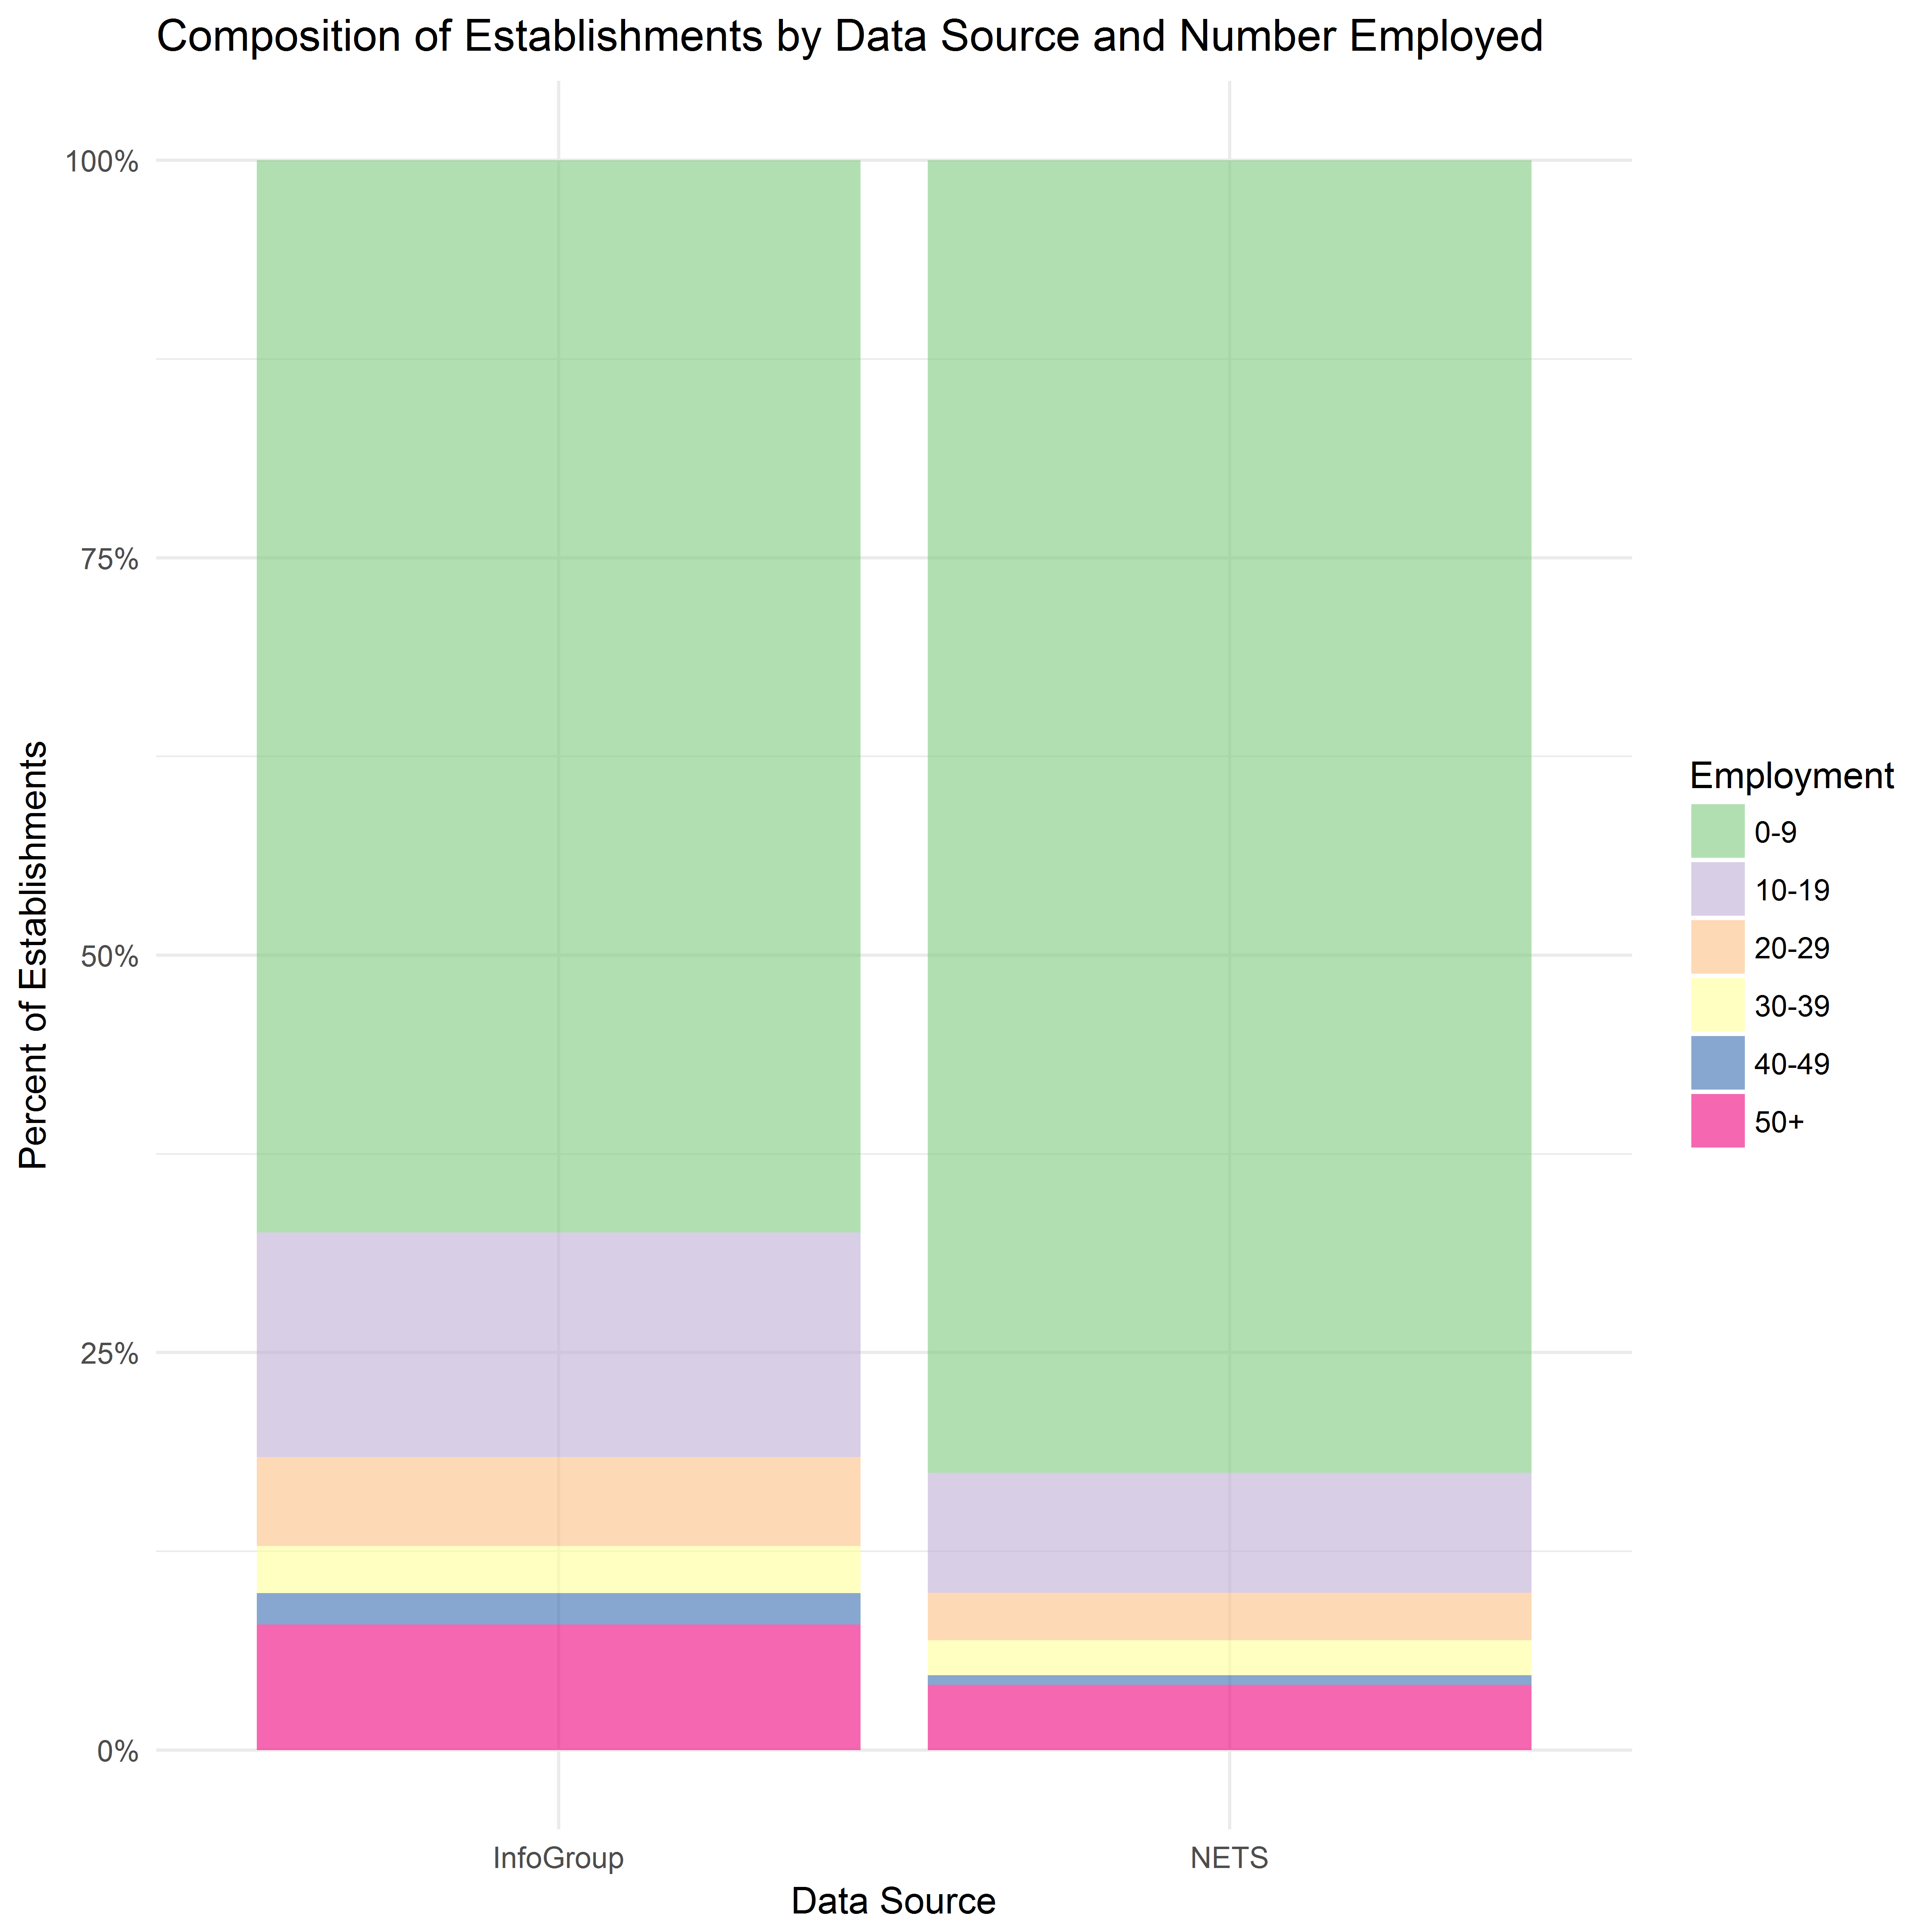
\includegraphics[width = 0.7\textwidth]{employmentComposition}
	\caption{Percentage of Establishments at Six Employment Levels.}
\end{figure}
\section{One-to-One Comparison of InfoUSA Sample to NETS Data}
For the random sample of 143 InfoUSA records, we manually matched the InfoUSA firms to their counterparts in the NETS dataset. We found 72 matches in total. Of these, there were:
\begin{itemize}
	\item 44 instances where InfoUSA reported more employees than NETS for the same establishment;
	\item 18 instances where NETS reported more employees than InfoUSA for the same establishment; and
	\item 10 instances where employment was the same in both NETS and InfoUSA.
\end{itemize}
The results indicate that, while InfoUSA has fewer overall records, it tends to report more employees than NETS for identical establishments. The average absolute percentage difference (see Footnote 3) between NETS and InfoUSA employment was 79.32\%, and the median was 66.67\%.
\section{Large Employers}
It is important to compare large employers in Conshohocken for at least three reasons: 1) They are the most visible employers in the area and therefore the easiest to verify; 2) They skew employment totals for individual geographic units, making it important that they are correctly geocoded; and 3) Small percentage differences between data sources for these establishments (i.e., between NETS and InfoUSA) can translate into large aggregate differences in employment for the area. Figure 2, \textit{Distribution of Establishments by Employment and Source}, shows the NETS and InfoUSA records with over 50 employees. Accounting for the overall difference in the number of records between NETS and InfoUSA, NETS reports establishments with approximately 50 employees more often than InfoUSA. This may drive the overall difference in employment tallies between NETS and InfoUSA for the study area.\par
\begin{figure}[h]
	\centering
	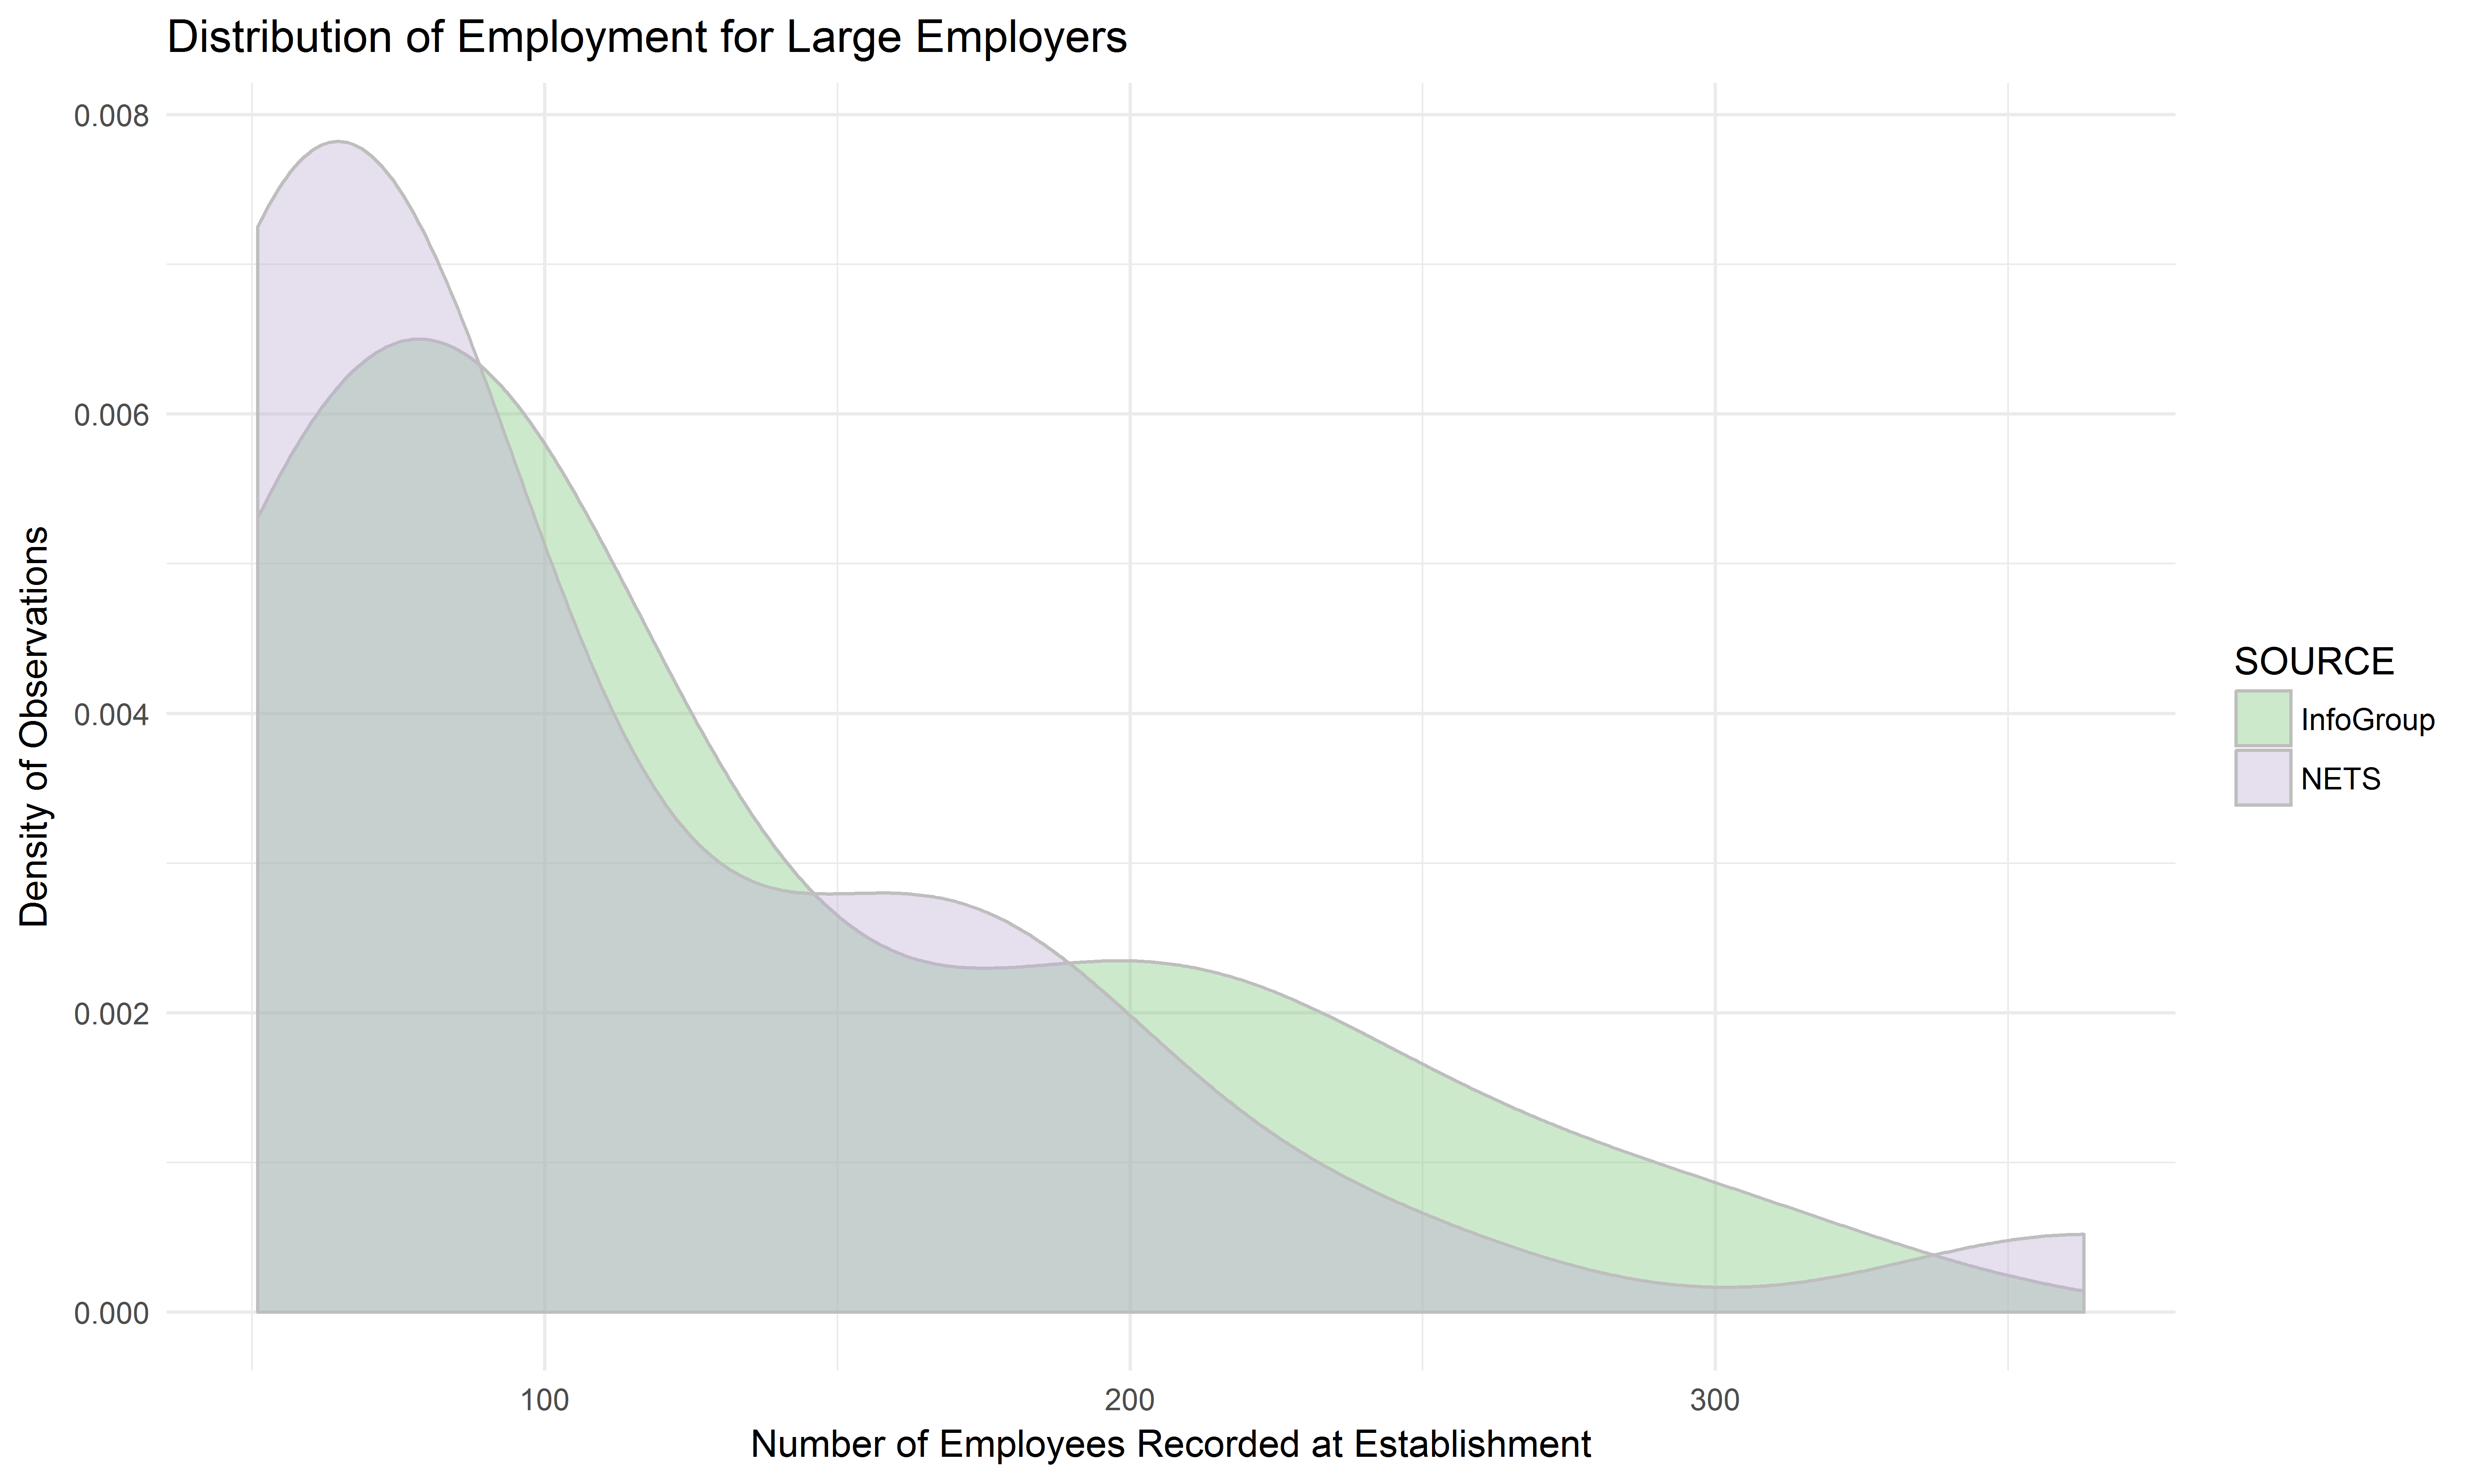
\includegraphics[width = 0.7\textwidth]{densityLgEmp}
	\caption{Distribution of Establishments by Employment and Source.}
\end{figure}
24 establishments in NETS and 19 in InfoUSA have a total reported number of employees exceeding 50. Of these, 7 large employers are present in both datasets. View Table 5, \textit{Differences in Employment for Seven Large Employers} for employment counts by employer and data source. In four instances, InfoUSA reported more employees than NETS for the same establishment. However, it is worth highlighting two employers: Employer D, where NETS reported 113 more employees than InfoUSA; and Employer E, where InfoUSA reported 118 more employees than NETS. Employer D occupies only one floor of a modest-sized office building: it is likely that the InfoUSA record is closer to the true number of employed in this instance. Furthermore, an online search shows that Employer E self-reports as having over 250 employees at this particular location, pointing again to the InfoUSA record as the more accurate record. Further investigation of the veracity of large employer records might indicate which of these data sources is more reliable in general.

\section{Overall Data Quality}
This section, as with the rest of the paper, assumes NETS data is already clean and consistent. To evaluate the overall quality of InfoUSA data, we manually cleaned the random sample of 143 InfoUSA records for Conshohocken.
\begin{enumerate}
	\item 2 of 143 (1.4\%) InfoUSA establishments had falsely duplicated names. In this case, the InfoUSA sample had one completely misplaced duplicate. A record for a similarly named business located in Newtown Square---not Conshohocken---somehow made it into the Conshohocken dataset. This happened because the Newtown Square record \textit{has the wrong latitude and longitude}. In addition, the business does not appear to exist in Newtown Square, though it does exist in Conshohocken.
	\item 14 of 143 (9.8\%) establishments required address formatting cleanup, e.g. changing ``Cnshohckn'' to ``Conshohocken.''
	\item 4 of 143 (2.8\%) of addresses were P.O. boxes.
	\item 14 of 143 (9.8\%) had the exact same address and suite number. In one instance, 12 establishments shared the same suite, which is suspicious.
\end{enumerate}

\section{Tables}
\begin{table}[h]
	\begin{center}
		\begin{tabular}{ r | c c }
			& NETS & InfoUSA \\
			\hline
			\hline
			Total Number of Establishments & 637 & 304 \\
			\hline 
			No. Establishments > 0 Employees & 631 & 286 \\
			\hline 
			No. Establishments > 50 Employees & 24 & 19 \\
			\hline
			Proposed Sample Size (90\% CI, MOE $\pm$ 5\%) & 143 & --- \\
			\hline  
		\end{tabular}
	\end{center}
	\caption{General Properties of NETS and InfoUSA Data for Conshohocken.}
\end{table}
\begin{table}[h]
	\begin{center}
		\begin{tabular}{ r | c c c }
			Tract GEOID & NETS & InfoUSA & LEHD \\
			\hline
			\hline
			42091204102 & 0 & 655 & 22 \\
			\hline 
			42091204200 & 5780 & 4167 & 4931 \\
			\hline 
			42091205906 & 0 & 48 & 178 \\
			\hline
			\hline
			TOTAL & 5780 & 4870 & 5131 \\
			\hline
		\end{tabular}
	\end{center}
	\caption{Differences in Employment, Tract Level.}
\end{table}
\begin{table}[h]
	\begin{center}
		\begin{tabular}{ r | c c c }
			Block Group GEOID & NETS & InfoUSA & LEHD \\
			\hline
			\hline
			420912041021 & 0 & 655 & 22 \\
			\hline 
			420912042001 & 3913 & 3031 & 3996 \\
			\hline 
			420912042002 & 1867 & 1136 & 935 \\
			\hline 
			420912059062 & 0 & 48 & 178 \\
			\hline
			\hline
			TOTAL & 5780 & 4870 & 5131 \\
			\hline
		\end{tabular}
	\end{center}
	\caption{Differences in Employment, Block Group Level.}
\end{table}
\clearpage
\begin{table}[h]
	\begin{center}
		\begin{tabular}{ p{1.5in} | p{1.25in} p{1.25in} p{1.25in} }
			Block Group GEOID & NETS & InfoUSA & LEHD \\
			\hline
			\hline
			Geocoding Accuracy & 2/3. Have previously cleaned dataset. & 1/3. Cannot import existing info from NETS. & 0/3. Census Geocoder, noise added.\\
			\hline 
			Presence of Duplicates & 1/3. Prevalent. & 1/3. Prevalent. & 0/3. Not available.\\
			\hline 
			Available SIC/NAICS Codes & 3/3. Highly detailed. & 3/3. Highly detailed. & 1/3. 2-digit NAICS.\\
			\hline
			Accurate Employment Count & 1/3. Cannot determine veracity. & 1/3. Cannot determine veracity. & 1/3. Noise added to block-level data.\\
			\hline
			Update Frequency & 1/3. 2015 release occurred Sept. 2018. & 3/3. Can request newest data anytime. & 1/3. No release calendar. \\
			\hline
			Establishment Level & 3/3. Available. & 3/3. Available. & 0/3. Not available.\\
			\hline
			Cost & 2/3. Affordable. & 1/3. Expensive. & 3/3. Free. \\
			\hline
			\hline
			\textbf{TOTAL} & 13/21 & 13/21 & 6/21 \\
			\hline
		\end{tabular}
	\end{center}
	\caption{DVRPC Assessment of Data Sources.}
\end{table}
\begin{table}[h]
	\begin{center}
		\begin{tabular}{ r | c c }
			Employer & NETS & InfoUSA \\
			\hline
			\hline
			A & 56 & 75 \\
			\hline 
			B & 56 & 64 \\
			\hline 
			C & 171 & 165 \\
			\hline
			D & 363 & 250 \\
			\hline 
			E & 182 & 300 \\
			\hline 
			F & 138 & 110 \\
			\hline 
			G & 60 & 75 \\
			\hline
		\end{tabular}
	\end{center}
	\caption{Differences in Employment for Seven Large Employers.}
\end{table}
\clearpage
\pagestyle{empty}
\begin{table}
	\begin{center}
		\begin{tabular}{ r | c c c c c c }
			Block GEOID & NETS & InfoUSA & LEHD & NETS x IG & NETS x LEHD & IG x LEHD \\
			\hline
			\hline
			420912041021003 & 0 & 655 & 22 & Yes & Yes & Yes \\
			\hline 
			420912042001006 & 72 & 0 & 0 & Yes & Yes & No \\
			\hline 
			420912042001008 & 430 & 1071 & 621 & No & No & No \\
			\hline 
			420912042001009 & 880 & 427 & 475 & No & No & No \\
			\hline 
			420912042001011 & 1056 & 551 & 417 & No & No & No \\
			\hline 
			420912042001012 & 858 & 24 & 0 & Yes & Yes & Yes \\
			\hline 
			420912042001014 & 33 & 34 & 161 & No & Yes & Yes \\
			\hline 
			420912042001015 & 1 & 0 & 0 & Yes & Yes & No \\
			\hline 
			420912042001016 & 41 & 44 & 55 & No & No & No \\
			\hline 
			420912042001018 & 110 & 24 & 33 & Yes & Yes & No \\
			\hline 
			420912042001019 & 2 & 0 & 0 & Yes & Yes & No \\
			\hline 
			420912042001021 & 60 & 57 & 101 & No & No & No \\
			\hline 
			420912042001022 & 44 & 44 & 0 & No & Yes & Yes \\
			\hline 
			420912042001034 & 63 & 176 & 2 & No & Yes & Yes \\
			\hline 
			420912042001035 & 93 & 493 & 835 & Yes & Yes & No \\
			\hline 
			420912042001037 & 4 & 5 & 1263 & No & Yes & Yes \\
			\hline 
			420912042001038 & 8 & 0 & 0 & Yes & Yes & No \\
			\hline 
			420912042001039 & 3 & 0 & 1 & Yes & Yes & Yes \\
			\hline 
			420912042001040 & 25 & 17 & 7 & No & Yes & No \\
			\hline 
			420912042001041 & 1 & 0 & 0 & Yes & Yes & No \\
			\hline 
			420912042001048 & 126 & 64 & 25 & No & Yes & No \\
			\hline 
			420912042001054 & 1 & 0 & 0 & Yes & Yes & No \\
			\hline 
			420912042001056 & 2 & 0 & 0 & Yes & Yes & No \\
			\hline 
			420912042002000 & 317 & 287 & 155 & No & No & No \\
			\hline 
			420912042002002 & 86 & 27 & 0 & Yes & Yes & Yes \\
			\hline 
			420912042002005 & 16 & 2 & 22 & Yes & No & Yes \\
			\hline 
			420912042002006 & 2 & 5 & 0 & No & Yes & Yes \\
			\hline 
			420912042002008 & 284 & 3 & 28 & Yes & Yes & Yes \\
			\hline 
			420912042002009 & 3 & 0 & 0 & Yes & Yes & No \\
			\hline 
			420912042002010 & 2 & 0 & 3 & Yes & No & Yes \\
			\hline 
			420912042002012 & 746 & 547 & 404 & No & No & No \\
			\hline 
			420912042002013 & 54 & 0 & 0 & Yes & Yes & No \\
			\hline 
			420912042002014 & 257 & 175 & 223 & No & No & No \\
			\hline 
			420912042002015 & 6 & 0 & 0 & Yes & Yes & No \\
			\hline 
			420912042002016 & 6 & 2 & 0 & Yes & Yes & Yes \\
			\hline 
			420912042002017 & 36 & 36 & 19 & No & No & No \\
			\hline 
			420912042002018 & 2 & 0 & 0 & Yes & Yes & No \\
			\hline 
			420912042002019 & 10 & 7 & 0 & No & Yes & Yes \\
			\hline 
			420912042002020 & 2 & 0 & 0 & Yes & Yes & No \\
			\hline 
			420912042002021 & 3 & 0 & 0 & Yes & Yes & No \\
			\hline 
			420912042002023 & 3 & 0 & 0 & Yes & Yes & No \\
			\hline 
			420912042002025 & 2 & 0 & 0 & Yes & Yes & No \\
			\hline 
			420912042002027 & 1 & 19 & 33 & Yes & Yes & No \\
			\hline 
			420912042002028 & 19 & 22 & 48 & No & No & No \\
			\hline 
			420912042002029 & 10 & 4 & 0 & No & Yes & Yes \\
			\hline 
			420912059062045 & 0 & 48 & 178 & Yes & Yes & Yes \\
			\hline
			\hline
			\textbf{TOTAL} & 5780 & 4870 & 5131 & 27 & 34 & 16 \\
			\hline
		\end{tabular}
	\end{center}
	\caption{Differences in Employment, Block Level.}
\end{table}
\end{document}